%----------------------------------------------------------------------------------------
%	LEFT COLUMN
%----------------------------------------------------------------------------------------

\begin{minipage}[t]{0.33\textwidth} % The left column takes up 33% of the text width of the page

\section{Profile}
\tikz[remember picture] 
\node[circle,xshift=8cm, yshift=0cm, opacity=0.9] {
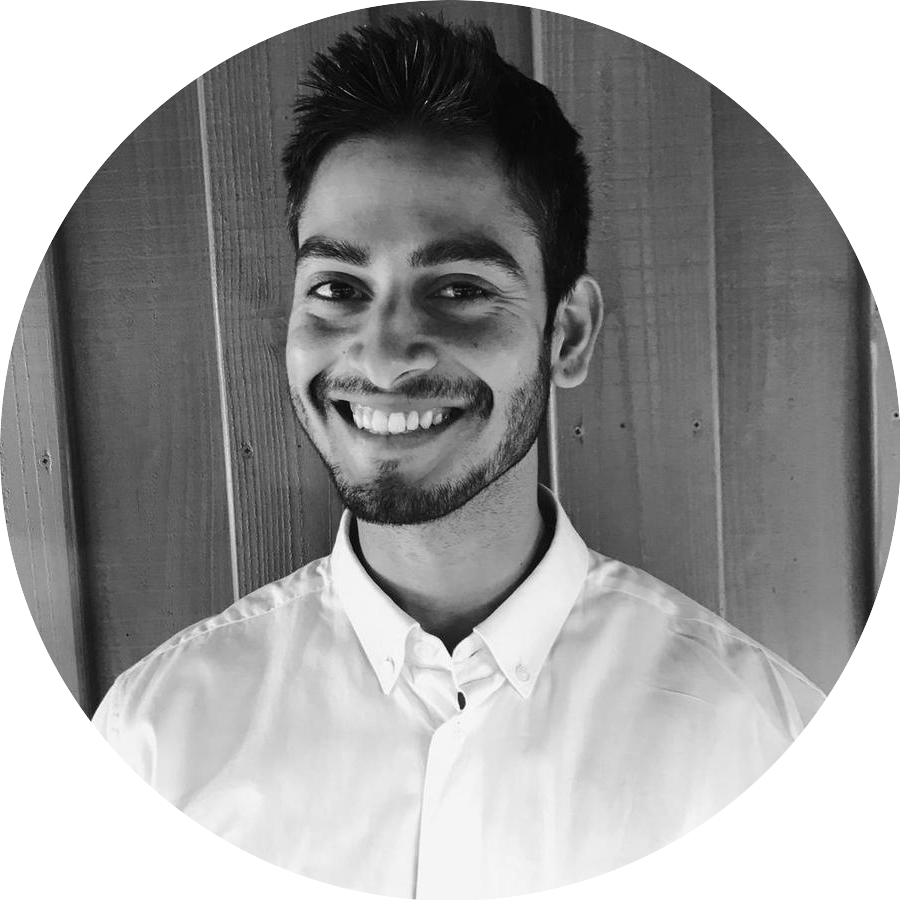
\includegraphics[width=2.8cm,height=3.0cm]{nbhushanCircle.png}
};

\emph{Curious about a data-driven world,\\ I spend my time connecting the dots\\ between engineering, data science \& AI,\\ and behavioural sciences.}

\vspace{8pt}

\section{Education} 
\runsubsection{PhD}
\descript{| data science}
\location{University of Groningen \\ Netherlands |  June 2020}
\vspace{\topsep} % Hacky fix for awkward extra vertical space
\vspace{1pt}
\begin{tightitemize}
\item topics: additive models, \\time series, graphical models,\\ causal inference
\item developed models to explore, understand, and predict the\\ human dimension of the\\ energy transition
\item advisors: \href{https://www.rug.nl/staff/e.m.steg/}{linda steg}, \href{https://www.rug.nl/staff/c.j.albers//}{casper albers} 
\end{tightitemize}
\vspace{7pt}

\runsubsection{MSc}
\descript{| Artificial Intelligence}
\location{Maastricht University\\Netherlands | 2013}
\begin{tightitemize}
\item foundations in \\probabilistic modelling 
\item relevant courses: data mining \& machine learning,text mining,\\and multi-agent systems 
\end{tightitemize}
\vspace{7pt}

\runsubsection{BE}
\descript{| Electrical engineering}
\location{MSRIT | Bangalore, India | 2009}
\begin{tightitemize}
\item foundations in energy systems 
\item relevant courses: \\applied mathematics,\\ control theory, \\energy technology,\\and power systems analysis
\end{tightitemize}
\vspace{8pt}

\sectionspace % Some whitespace after the section


%------------------------------------------------
% Coursework
%------------------------------------------------
\sectionspace % Some whitespace after the section
\end{minipage} % The end of the left column
\hfill
%
%----------------------------------------------------------------------------------------
%	RIGHT COLUMN
%----------------------------------------------------------------------------------------
%
\begin{minipage}[t]{0.66\textwidth} % The right column takes up 66% of the text width of the page

%------------------------------------------------
% Experience
%------------------------------------------------
\section{Experience}

\runsubsection{Breda University of Applied Sciences}
\descript{| data science educator}
\location{april 2021 - now | Breda, The Netherlands}
\vspace{\topsep}
\begin{tightitemize}
\item design and execute a project-based bachelor study program in applied data science and AI in close collaboration with the industry.
\end{tightitemize}
\sectionspace

\runsubsection{Bosch Transmission Technology BV.}
\descript{| data science consultant}
\location{dec 2019 - april 2021 | Tilburg, The Netherlands}
\vspace{\topsep}
\begin{tightitemize}
\item external contractor via TMC Data Science BV.
\item data science \& AI - computer vision, predictive modelling \& root cause analysis.
\item BI - developed reports and dashboards using Microsoft Power BI.
\item initiated, organised, and delivered interactive workshops on AI and data science.
\end{tightitemize}
\sectionspace

\runsubsection{University of Groningen}
\descript{| researcher, consultant, lecturer } 
\location{September 2015 - September 2019 | Groningen, Netherlands}
\vspace{\topsep} % Hacky fix for awkward extra vertical space
\begin{tightitemize}
\item lecturer: statistical inference and regression modelling (>100 students).
\item developed tools to evaluate the effectiveness of energy efficiency programs and guide energy policy.
%\item applied models to explore, understand, and predict human behaviour.
\item researched the applicability of causal Bayesian networks to solve problems of causal inference in psychology.
\item initiated, collaborated and delivered on four multi-disciplinary data science projects.
\item supervised  bachelor thesis projects.
\end{tightitemize}

\sectionspace % Some whitespace after the section


%------------------------------------------------

\runsubsection{TU Eindhoven}
\descript{| smart energy systems consultant trainee}
\location{January 2014 - June 2015 | Eindhoven, Netherlands}
\begin{tightitemize}
\item multi-disciplinary professional training on sustainable technologies and applications to the built environment.
\item developed and researched innovative business models to fund\\ the energy transition.
\end{tightitemize}
\sectionspace % Some whitespace after the section

%------------------------------------------------

\runsubsection{Xerox Research}
\descript{| machine learning intern}
\location{June 2012 – September 2013 | Grenoble, France}
\begin{tightitemize}
\item researched and implemented an extension to the hidden Markov model to describe sequential data where the state duration follows a truncated distribution and the dynamics of the model depend on whether the truncation was reached.
\item developed a smart energy management system for electrical devices. 
%\item delivered production-ready \href{https://github.com/nbhushan/QDHMMrepo}{code} in Python to learn real-time performance indicators of electrical devices. 
\end{tightitemize}
\sectionspace % Some whitespace after the section

%------------------------------------------------
% Some whitespace after the section
%----------------------------------------------------------------------

\section{tools \& skills}
\textbf{expert}: Python \textbullet{} R \textbullet{} \LaTeX{}\\ 
\textbf{proficient}: \textbullet{} SQL 
\textbf{algorithms}\\\textbullet{} data visualisation \& business intelligence \\\textbullet{} regression, classification \& clustering\\ \textbullet{} causal inference (XAI) \& deep learning \\ \textbullet{} time-series modelling \& forecasting\\

\end{minipage} % The end of the right column
\vspace*{\fill}
\center{\textcolor{gray}{1/2}}


